\rev{\subsection{Sensitivity to hyperparameters and simulator parameters}\label{sec:sensitivity}\revnote{R3.2}
This subsection quantifies how the results depend on the parameters that were fixed a priori (Section~\ref{sec:paramsel}).

\emph{Agent hyperparameters.} Table~\ref{tab:component} reports AA-DQN for three learning rates, three discount factors, four history lengths, a recurrent encoder and with each stabilisation component removed (three seeds each). Varying the learning rate from $5\times10^{-4}$ to $10^{-3}$ or the discount factor from $0.99$ to $0.999$ changes the return by less than 0.1 (\compAADQNLrOneeThreeRet{} and \compAADQNGZeroNineNineNineRet{} versus \compAADQNRet). Two settings are worse by about 0.45: a learning rate of $10^{-4}$ (\compAADQNLrOneeFourRet), which learns too slowly for the 5000-episode budget, and a discount factor of $0.95$ (\compAADQNGZeroNineFiveRet), whose effective horizon of about 20 slots (3.3~h) is shorter than the day, so that consequences of decisions for late deadlines are discounted away. All these settings remain well above the vanilla DQN (\DQNReturn). The history length has the largest effect ($k=1$: \compAADQNNoHistRet; $k=8$: \compAADQNKEightRet), as discussed in Section~\ref{sec:component}. AA-PPO used untuned default settings and nevertheless achieved the best results, so its performance is not the product of hyperparameter search. The reward weight $\lambda$ is analysed in Section~\ref{sec:pareto}.

\emph{Simulator parameters.} Each of the seven cognitive parameters ($\alpha$, $\beta$, $\delta$, $\eta$, $\kappa$, $\gamma$, $\phi$) was decreased and increased by 30\%, one at a time, and every trained policy and tuned rule was evaluated, without retraining or re-tuning, on the 500 test days under each of the 14 perturbed models (Table~\ref{tab:simsens}, Fig.~\ref{fig:simsens}). This is a conservative test, because the learned policies and the rules are applied to dynamics they were not optimised for. The parameters that govern the depletion of attention ($\alpha$), the accumulation of fatigue ($\delta$) and its effect on throughput ($\kappa$) change the attainable return the most (by 1.2--1.4 for AA-PPO), whereas the circadian amplitude $\gamma$ and the fatigue coupling $\phi$ have small effects. The fixed work--rest cycle of EDF-Periodic is the most sensitive policy (a range of 2.3 for $\alpha$), because it cannot adapt the amount of rest. The ranking of the methods is remarkably stable. Both AA-PPO variants exceed the best rule in all \ssNConds{} perturbed models (AA-PPO by at least \ssPPOGapMin; best learned policy minus best rule between \ssGapMin{} and \ssGapMax), and the intensity-only AA-DQN does so in \ssAADQNThreeactWins{} of them. The hybrid AA-DQN, which ties with the best rule in the nominal model, falls slightly behind it in most perturbed models (\ssAADQNWins{} of \ssNConds{} wins; at worst by $\ssAADQNGapMin$). The main conclusions therefore do not hinge on the particular parameter values in Table~\ref{tab:params}, although, as for any simulation study, they cannot replace calibration with real data (Section~\ref{sec:limitations}).

\begin{table}[!htbp]
\centering
\caption{Zero-shot sensitivity to the cognitive parameters: return on 500 test days when one parameter is changed by $\pm30\%$ (learned policies: mean of ten seeds; rules: parameters tuned in the nominal model). The last column gives the return of the best learned policy minus that of the best rule. Bold marks the best method in each row.}
\label{tab:simsens}
\small
\resizebox{\textwidth}{!}{\begin{tabular}{llccccccccc}
\toprule
Parameter & Change & AA-PPO & AA-PPO, intensity & AA-DQN & AA-DQN, intensity & SPT-Threshold & SPT-Periodic & EDF-Periodic & EDF & Best learned $-$ best rule \\
\midrule
Nominal & -- & 13.04 & \textbf{13.20} & 12.17 & 12.61 & 12.30 & 12.25 & 11.41 & 4.24 & +0.89 \\
Attention depletion $\alpha$ & $-30\%$ & 13.77 & \textbf{13.91} & 12.93 & 13.42 & 12.73 & 12.65 & 12.57 & 6.56 & +1.18 \\
 & $+30\%$ & 12.44 & \textbf{12.50} & 11.46 & 11.87 & 11.88 & 11.71 & 10.25 & 2.37 & +0.61 \\
Attention recovery $\beta$ & $-30\%$ & \textbf{12.48} & 12.47 & 11.60 & 11.93 & 11.82 & 11.60 & 10.05 & 4.24 & +0.65 \\
 & $+30\%$ & 13.50 & \textbf{13.67} & 12.57 & 13.07 & 12.59 & 12.67 & 12.44 & 4.24 & +1.00 \\
Fatigue accumulation $\delta$ & $-30\%$ & 13.73 & \textbf{13.85} & 12.85 & 13.22 & 12.98 & 12.83 & 12.58 & 5.55 & +0.86 \\
 & $+30\%$ & 12.48 & \textbf{12.55} & 11.55 & 12.03 & 11.74 & 11.64 & 10.42 & 3.23 & +0.81 \\
Fatigue recovery $\eta$ & $-30\%$ & 12.61 & \textbf{12.65} & 11.80 & 12.21 & 11.92 & 11.80 & 10.68 & 4.24 & +0.73 \\
 & $+30\%$ & 13.38 & \textbf{13.52} & 12.44 & 12.87 & 12.58 & 12.55 & 12.10 & 4.24 & +0.95 \\
Fatigue penalty $\kappa$ & $-30\%$ & 13.81 & \textbf{13.90} & 12.97 & 13.41 & 12.81 & 12.64 & 12.49 & 5.16 & +1.09 \\
 & $+30\%$ & 12.39 & \textbf{12.42} & 11.28 & 11.72 & 11.80 & 11.71 & 10.40 & 3.32 & +0.62 \\
Circadian amplitude $\gamma$ & $-30\%$ & 13.24 & \textbf{13.47} & 12.33 & 12.82 & 12.43 & 12.41 & 11.81 & 4.49 & +1.04 \\
 & $+30\%$ & 12.85 & \textbf{12.95} & 12.01 & 12.39 & 12.14 & 11.98 & 11.01 & 3.99 & +0.81 \\
Fatigue coupling $\phi$ & $-30\%$ & 13.12 & \textbf{13.27} & 12.28 & 12.71 & 12.35 & 12.30 & 11.56 & 4.57 & +0.92 \\
 & $+30\%$ & 12.97 & \textbf{13.13} & 12.08 & 12.52 & 12.25 & 12.18 & 11.27 & 3.89 & +0.87 \\
\bottomrule
\end{tabular}}
\end{table}

\begin{figure}[!htbp]
\centering
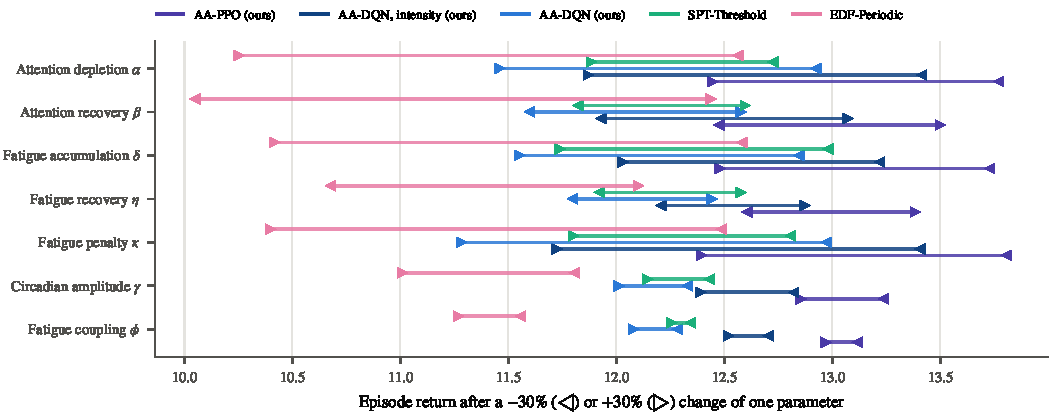
\includegraphics[width=\textwidth]{figures/fig_simsens.pdf}
\caption{Return of selected policies after a $-30\%$ ($\triangleleft$) or $+30\%$ ($\triangleright$) change of one cognitive parameter (500 test days, zero-shot). The learned policies stay ahead of the rules for every parameter.}
\label{fig:simsens}
\end{figure}
}
